\documentclass[aps,pre,preprint]{revtex4}
% \documentclass[aps,pre,twocolumn]{revtex4-1}
% \documentclass[aps,jcp,groupedaddress,twocolumn,unsortedaddress]{revtex4}

\usepackage{amsmath}
\usepackage{amssymb}
\usepackage[dvips]{graphicx}
\usepackage{color}
\usepackage{tabularx}
\usepackage{algorithm}
\usepackage{algorithmic}

\makeatletter
\makeatother

\newcommand{\recheck}[1]{{\color{red} #1}}
\newcommand{\redc}[1]{{\color{red} #1}}
\newcommand{\bluec}[1]{{\color{blue} #1}}
\renewcommand{\v}[1]{\textbf{\textit{#1}}}
\renewcommand{\d}[1]{\textsf{#1}}


\begin{document}

\title{Adaptive Resolution Simulation (AdResS): A smooth thermodynamic and structural transition from atomistic to coarse grained resolution and vice versa in a Grand Canonical fashion}
\author{Han Wang}
\affiliation{Institute for Mathematics, Freie Universit\"at Berlin, Berlin, Germany}
\author{Christof Sch\"utte}
\affiliation{Institute for Mathematics, Freie Universit\"at Berlin, Berlin, Germany}
\author{Luigi Delle Site}
\affiliation{Institute for Mathematics, Freie Universit\"at Berlin, Berlin, Germany}


\begin{abstract}
The AdResS method in Molecular Dynamics (MD) allows, in a Grand Canonical (GC) fashion, to change on-the-fly the number of degrees of freedom of a system, allowing to pass from atomistic (AT) to coarse-grained (CG) resolution and vice versa as a function of the position of the molecule in the simulation box. The coupling of resolutions is made in a thermodynamically consistent way, though, in the current formulation, in the region where the molecule changes resolution, neither thermodynamic nor structural properties can be preserved. Here we propose an extension of the method where basic thermodynamic and structural properties can be systematically controlled also in the transition region; this assures to have a very smooth change from one molecular representation to the other. Moreover we provide a rigorous argument which shows that if in the region where the molecules change resolution the radial distribution function is the same in the AT and CG region then the AT region, is from the statistical point of view, equivalent to a subsystem embedded in a larger full AT system, at least up to a second order approximation.    
\end{abstract}

\maketitle

\section{Introduction}
Bridging scales in condensed matter, material science of chemical physics is equivalent to describe the connection between local processes and the emerging global behaviour of the system and in this context, molecular simulation has the final aim of understanding the molecular origin of large scale properties. This can be viewed as a sort of process of zooming in (to the details) and zooming out (to the large scale properties) as pictorially illustrated in the example of Fig.\ref{zoom}. Standard molecular simulation techniques do not allow the zooming process in a concurrent fashion, that is considering different resolutions at the same time. Rather the zooming process is done in a sequential hierarchical way, in a bottom-up or top-down fashion \cite{annurev}. Ideally, a computational magnifying glass as in Fig.\ref{zoom} should be designed as an adaptive resolution approach. This means that it should: {\bf (1)} change molecular resolution in a region of space keeping the rest of the system at lower resolution; {\bf (2)} allow for the free exchange of molecule between the different regions, so that natural particle number fluctuations  are not arbitrarily suppressed; and {\bf (3)} the point (1) and (2) must occur under conditions of thermodynamic equilibrium which are the same as if the whole system was described at higher resolution only.
This implies that the temperature and particle density (at least) are the same in the AT and CG region, and are the same of a full AT simulation of reference \cite{annurev}. The computational advantages are obvious, simpler models requires less computational energies and thus can be more efficient. However, the real advantage of a method of this kind is in its conceptual consequences: it can in principle identify the essential degrees of freedom (DOF's) of a system and thus avoid to produce an excess of details which may overshadow the essential physics or chemistry of the system. A method with the characteristics outlined above is the Adaptive Resolution Simulation (AdResS) scheme \cite{jcp,pre} whose basic aspects are reported in the next section. In this work we propose an extension of the AdResS method which allows an even smoother transition from one resolution to the other. Based on such an extension we then give theoretical arguments which make the general theoretical framework more solid.
\begin{figure}
  \centering
  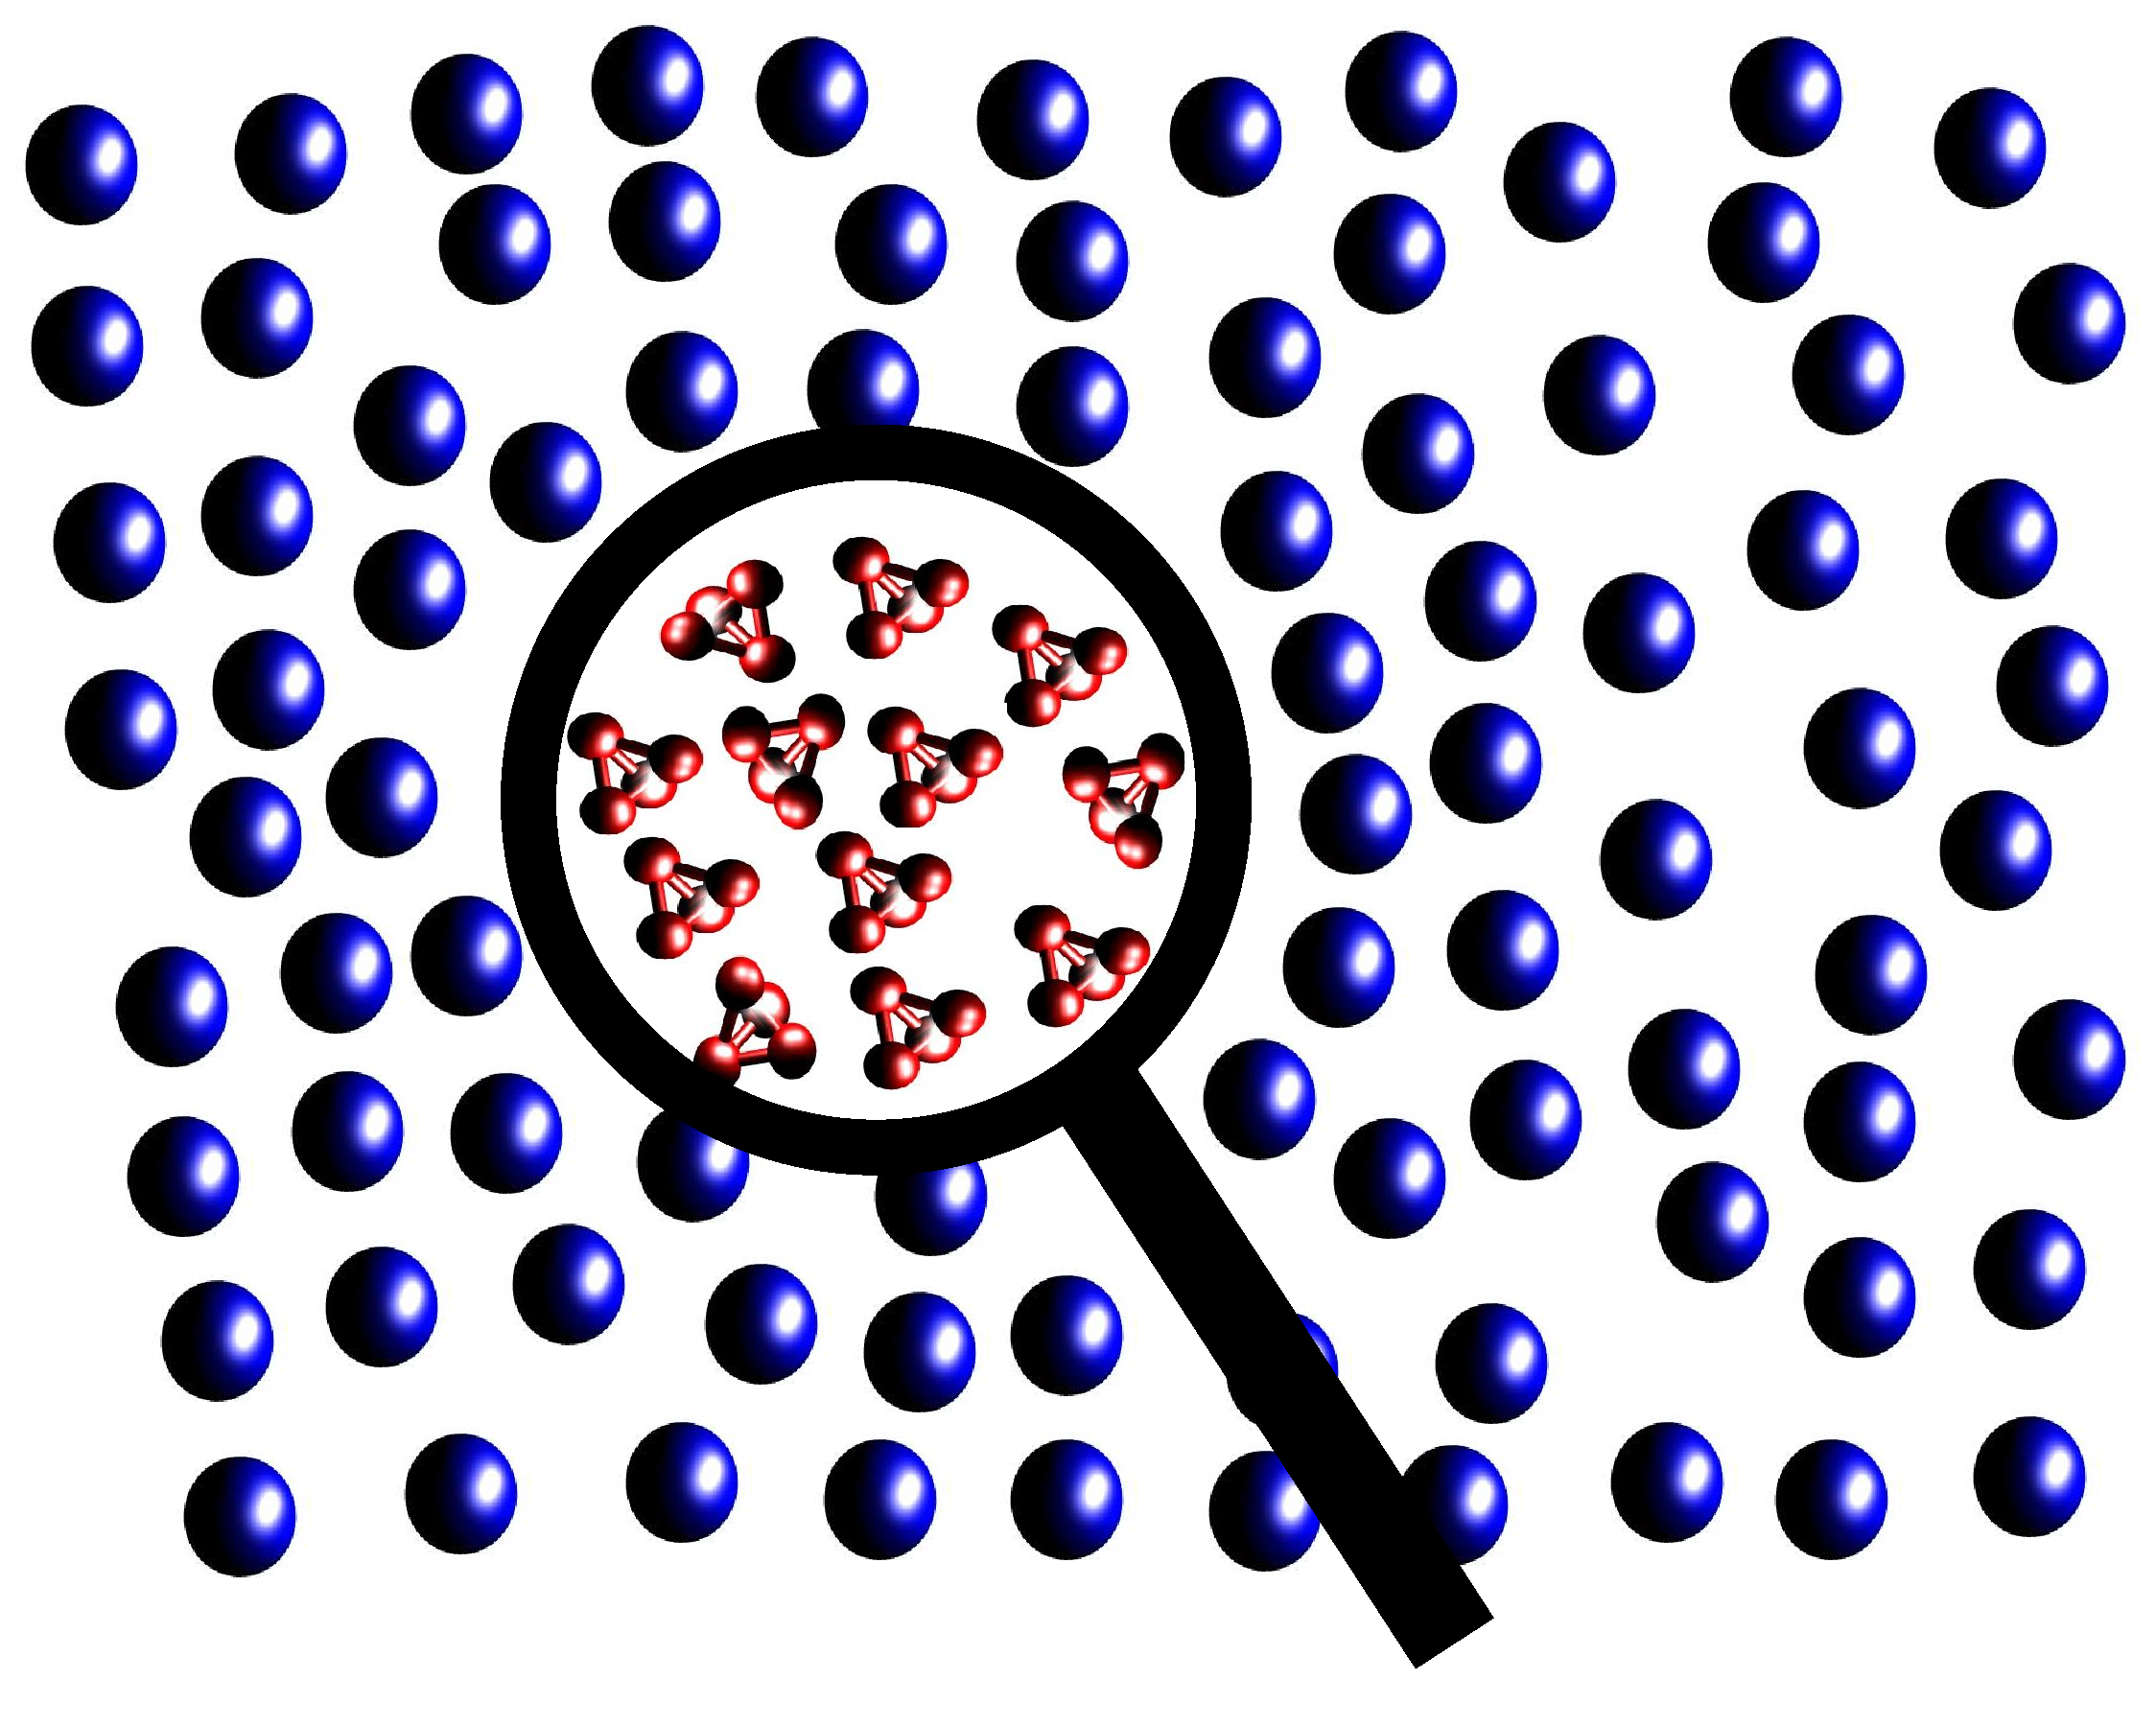
\includegraphics[angle=0,width=10cm]{zoom.eps}
  \caption{The magnifying glass illustrates the idea of zooming in to the AT scale to understand the molecular origin of the statistical properties of a liquid which at larger scale can be viewed as a collection of spheres, a resolution sufficient to represent the large scale behaviour.}
  \label{zoom}
\end{figure} 

\section{AdResS: Basic aspects}
The  AdResS method allows an on-the-fly interchange between the AT and coarse grained description (and vice versa) of the molecules according to their position in space. 
The two resolutions are coupled across scales by dividing the system into three parts (see also Fig.\ref{adapt}): {\bf (a)}
a high resolution region (AT) with atomistic details; {\bf (b)} a low resolution region (CG) with a simple-sphere
representation of molecules; and {\bf (c)} a transition region ($\Delta$) within which molecules continuously
adapt resolution through a space dependent interpolation of the high and low resolution intermolecular
forces:
\begin{figure}
  \centering
  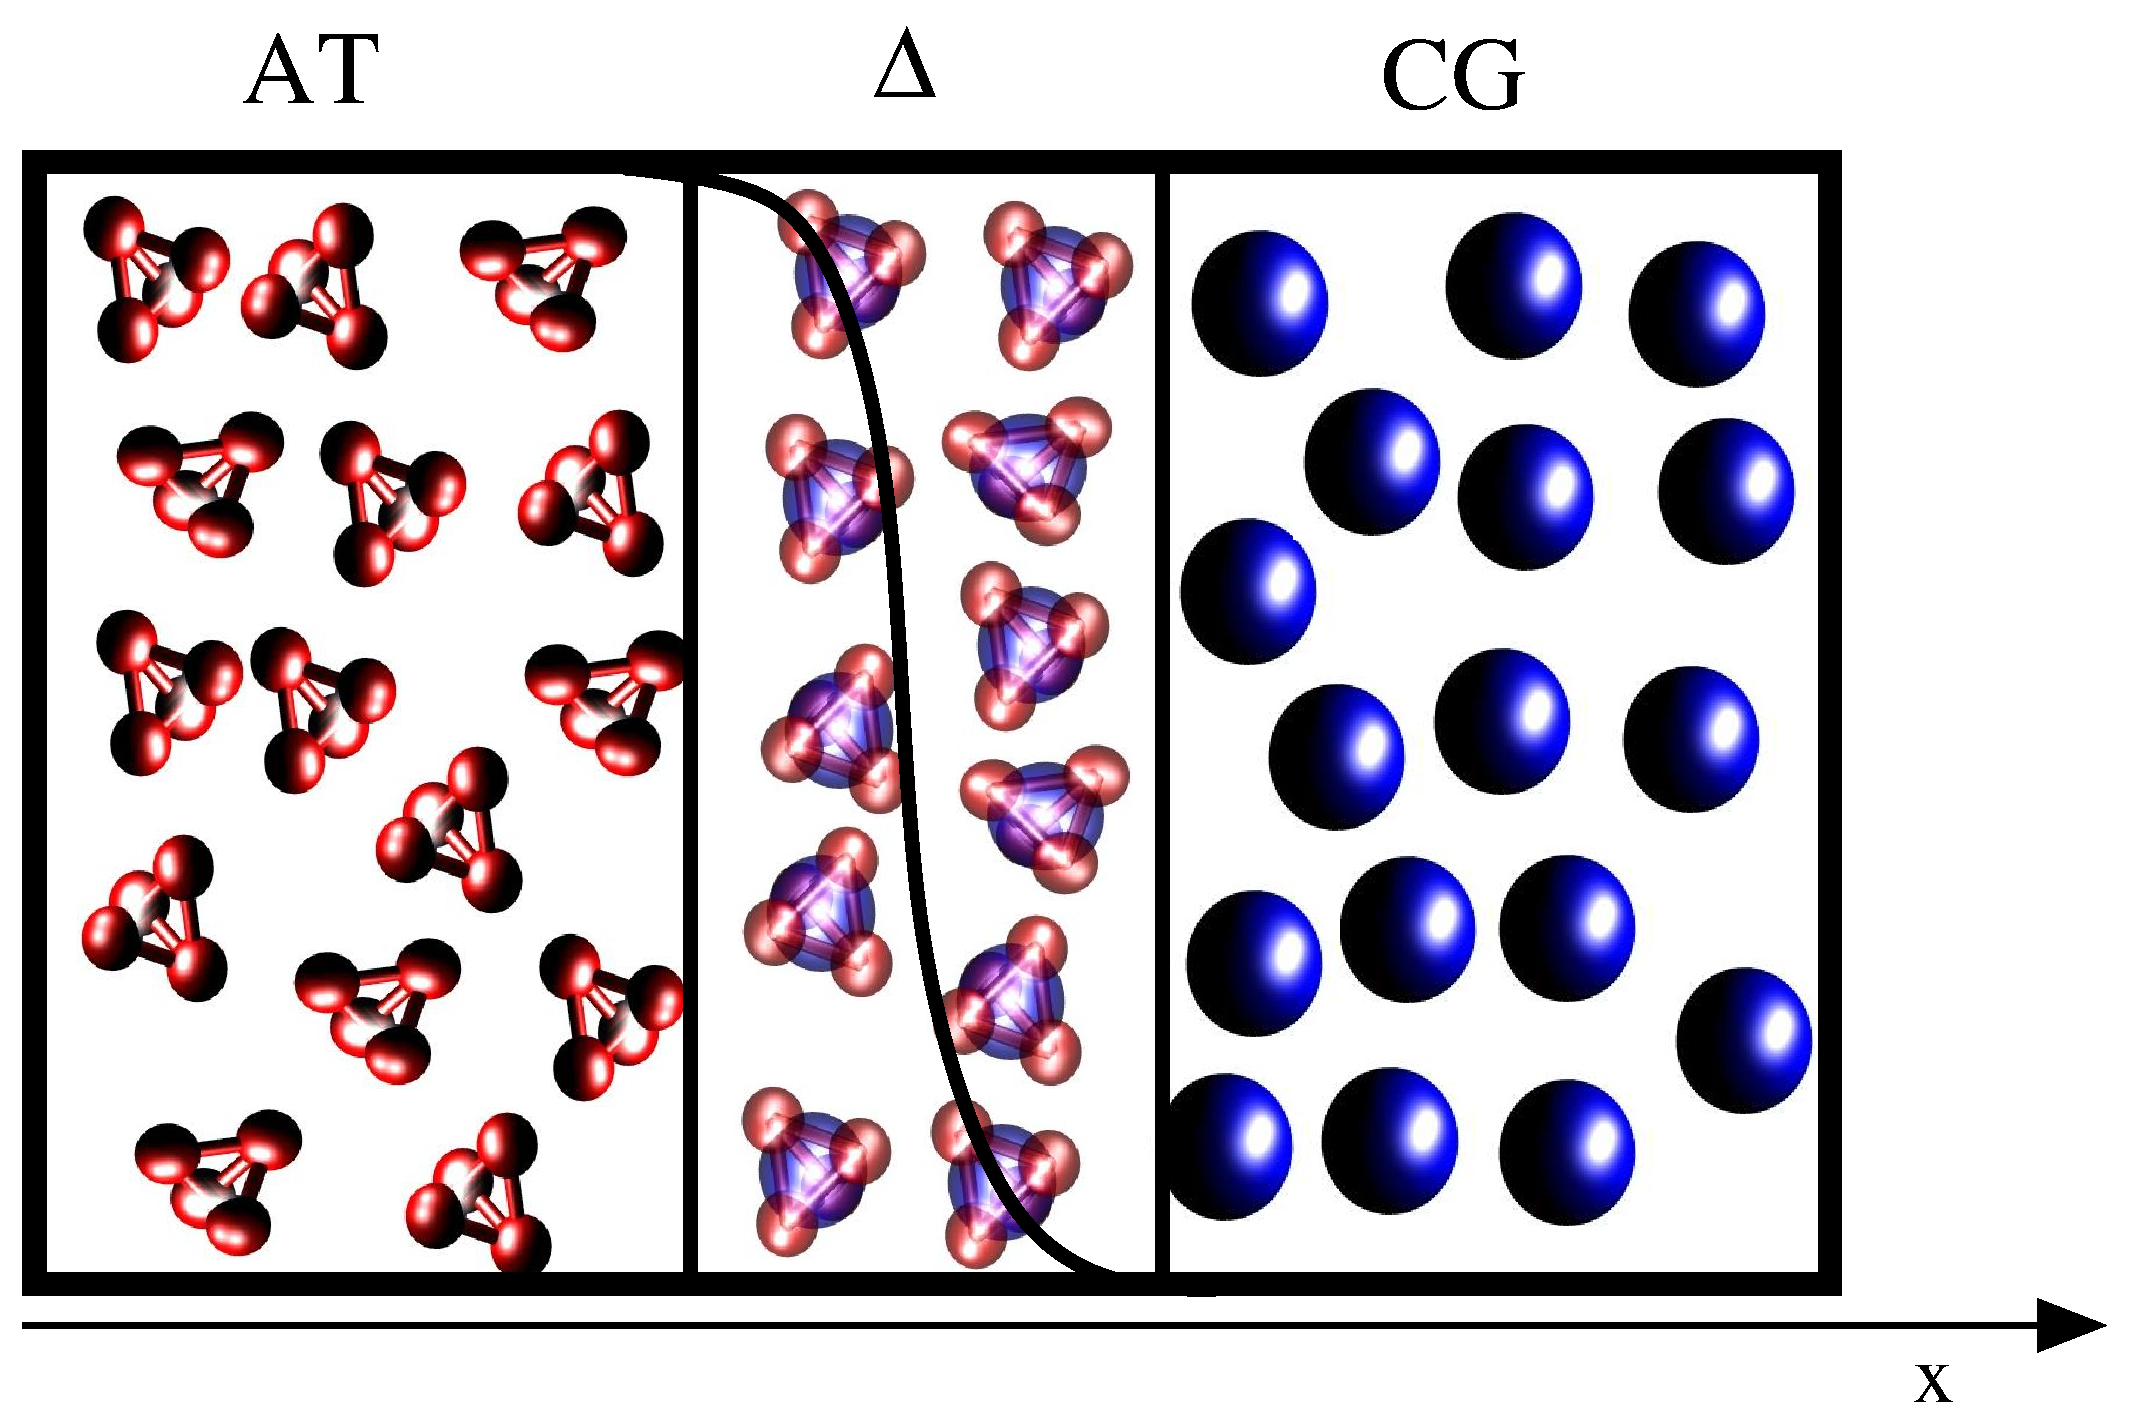
\includegraphics[angle=0,width=10cm]{adapt-pic.eps}
  \caption{Schematic representation of the adaptive simulation box. Molecules moving from the atomistic regio (AT) region slowly loose their resolution passing through continuous level of hybrid resolution in the transition region, $\Delta$, and then becoming spheres in the coarse-grained region (CG) (and vice versa). The example shown here consists of a liquid of tetrahedral molecules, that is the toy model used for developing the AdResS method \cite{jcp}. The region $\Delta$ in realistic applications should be much smaller than AT and CG region, here $\Delta$ is enlarged in order to make pictorially clear the hybrid resolution and the shape of $w(x)$.}
  \label{adapt}
\end{figure} 
\begin{equation}
{\v F}_{\alpha \beta}=w(x_\alpha)w(x_\beta){\v F}_{\alpha\beta}^{AT}+[1-w(x_\alpha)w(x_\beta)]{\v F}^{CG}_{\alpha\beta}
\label{force}
\end{equation}
where $\alpha$ and $\beta$ labels two molecules, ${\v F}_{\alpha\beta}^{AT}$ is the force derived from the AT potential and ${\v F}^{CG}_{\alpha\beta}$ is the force derived by the CG potential acting on the COMs, $w(x)$ is a function with value zero in the CG region, one in the AT and smooth and monotonic in the transition region $\Delta$. The standard form of $w(x)$ currently used in the AdResS scheme is:
\begin{align}\label{eqn:old-w}
  w(x) =
  \left\{
    \begin{array}{lcl}
      1 &\quad& x < d_{\textrm{AT}}\\
      \cos^2\big[\frac{\pi}{2(d_{{\Delta}})} (x - d_{\textrm{AT}})\big] && d_{\textrm{AT}}  < x < d_{\textrm{AT}} + d_{{\Delta}} \\
      0 && d_{\textrm{AT}} + d_{{\Delta}}  < x
    \end{array}
  \right.
\end{align}
where $d_{\textrm{AT}}$ and $d_{{\Delta}}$ are the size of the
atomistic and hybrid region, respectively and $x$ is the $x$-coordinate of the COM of a molecule measured along the $x$-axis as defined in Fig.\ref{adapt}.
The CG potential is derived from a reference full AT simulation and is such that it reproduces structural or thermodynamic properties of the reference full AT system; later we will discuss the coarse-graining procedure in more detail. The way the force of Eq.\ref{force} acts between the molecules is illustrated in Fig.\ref{inter}. 
\begin{figure}
  \centering
  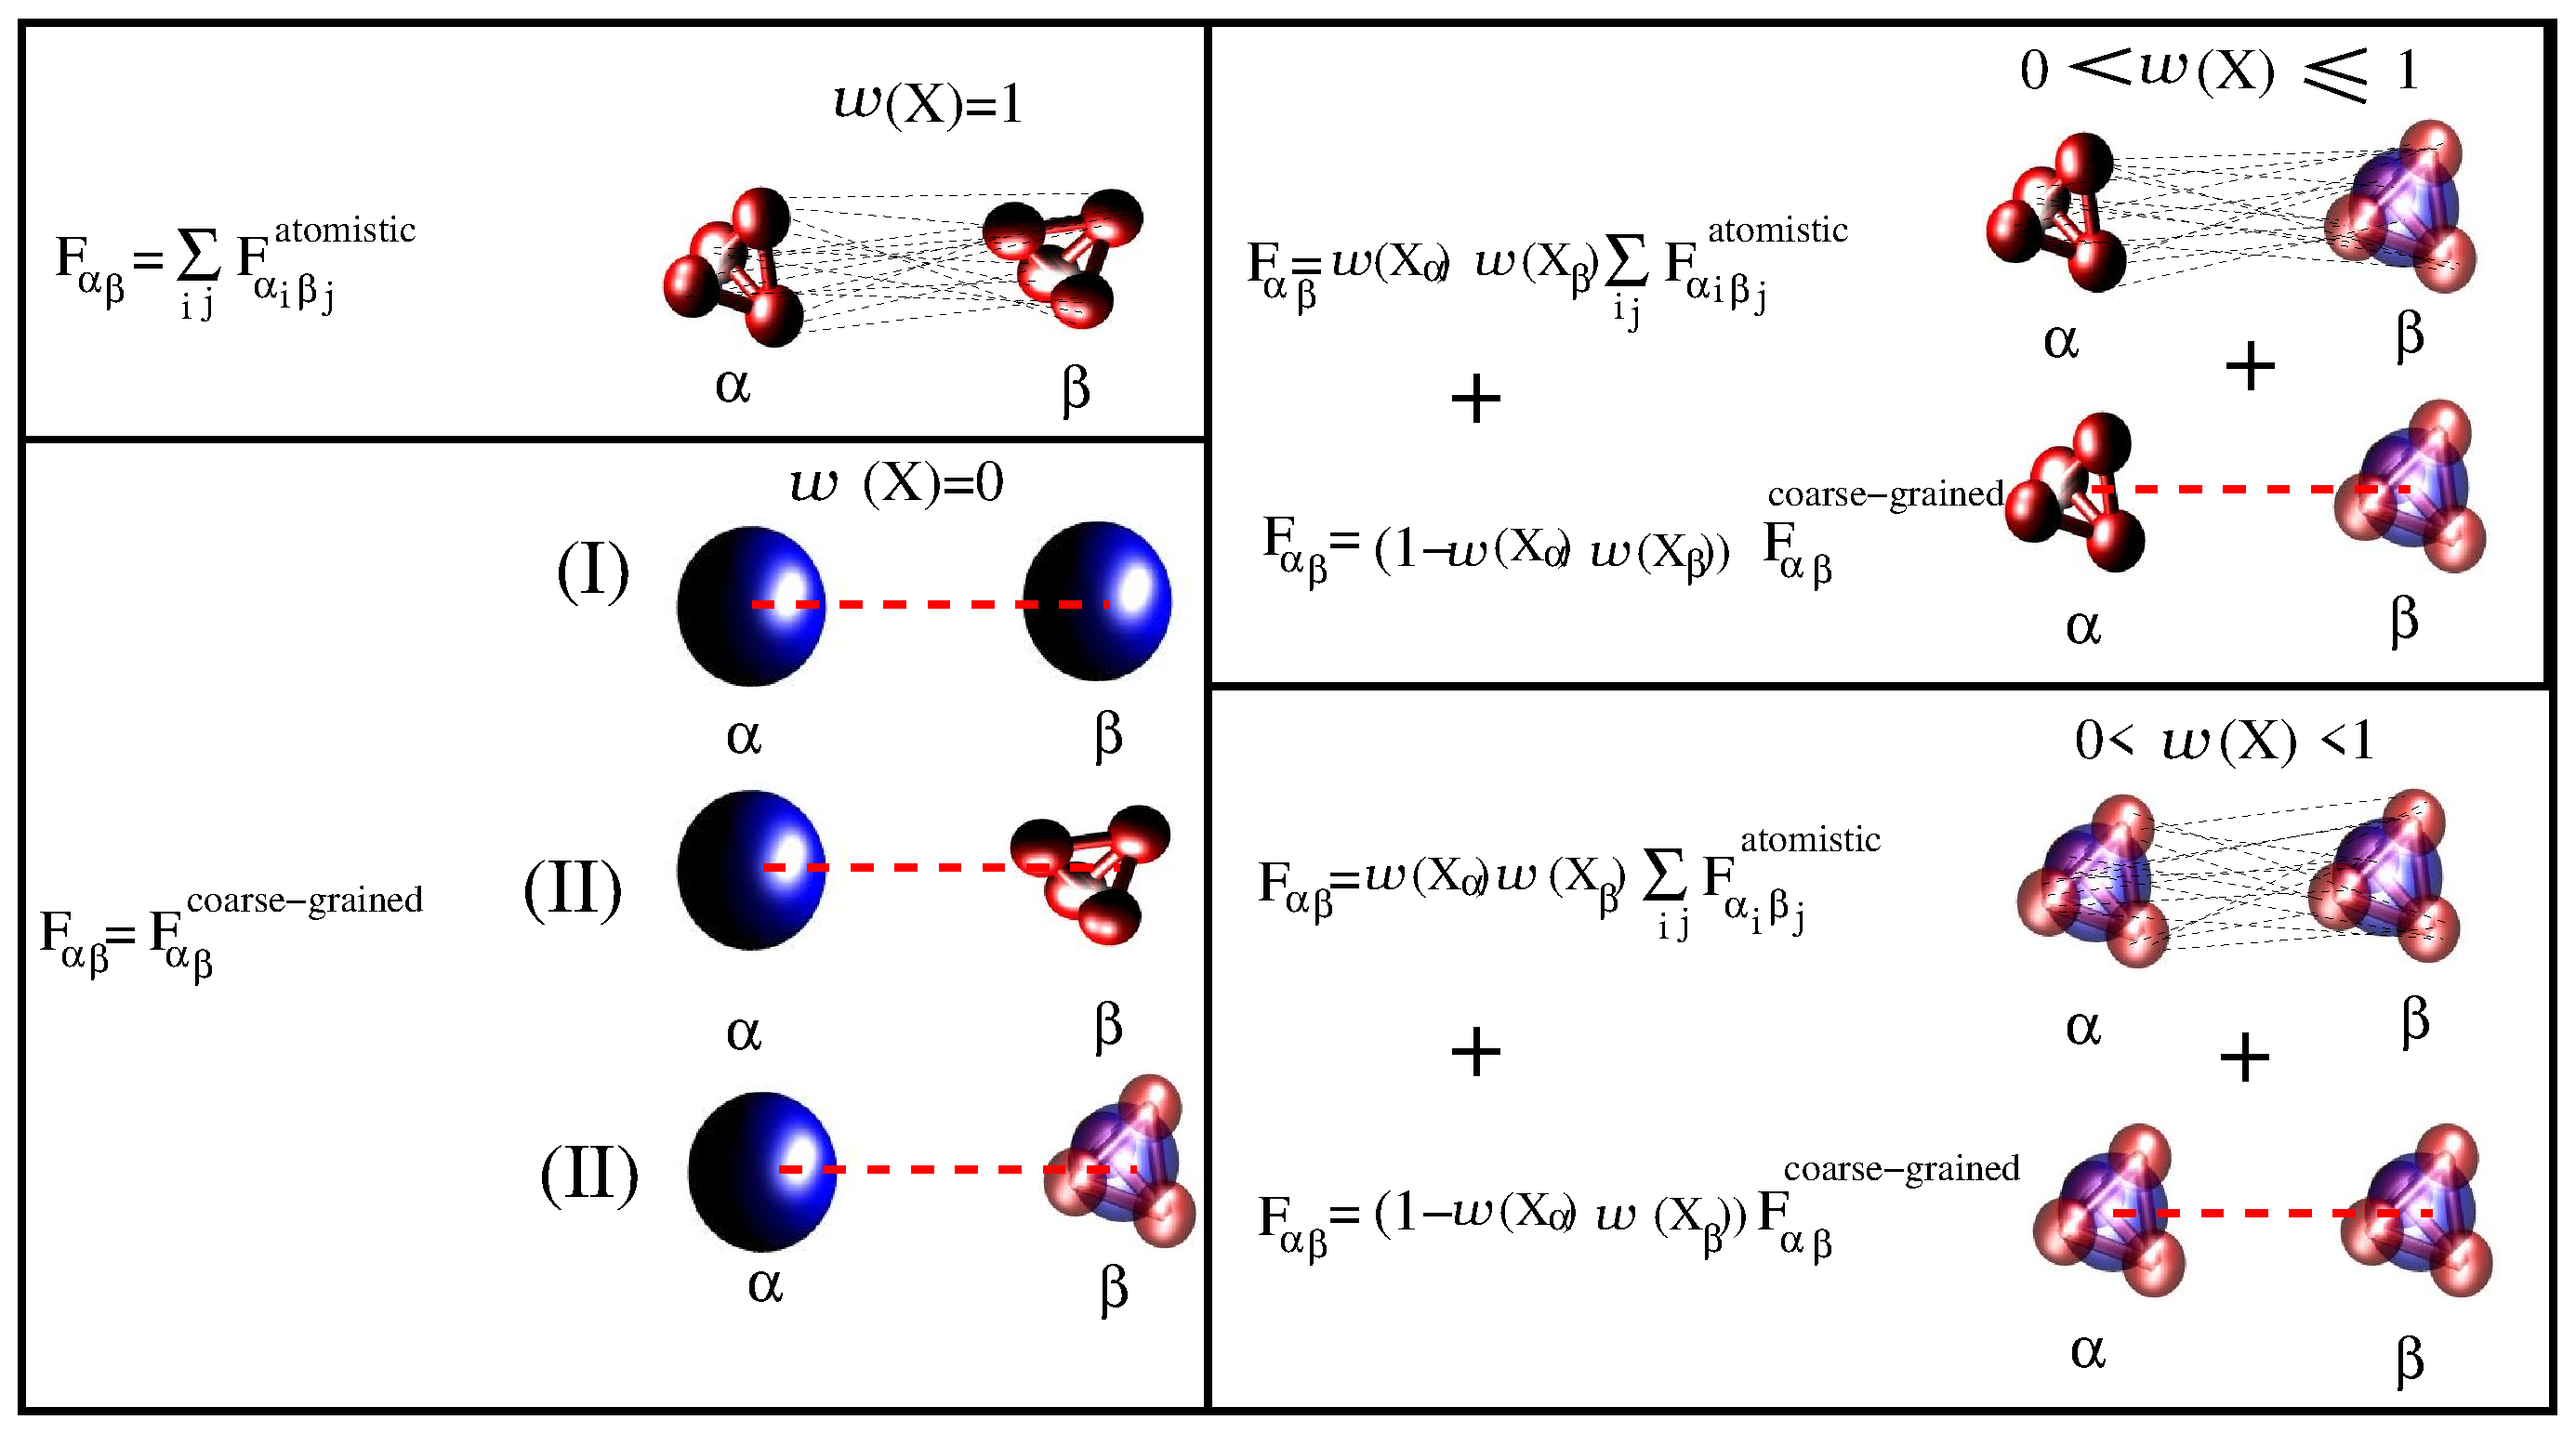
\includegraphics[angle=0,width=17cm]{force.eps}
  \caption{How ${\v F}_{\alpha,\beta}$ acts between the molecules. Two AT molecules(i.e. $w(x)=1$)  interact as standard AT molecules, that is each atom $i$ of $\alpha$ with each atom $j$ of $\beta$. Two GC molecules, $w(x)=0$ interact via the COM (no atomistic DOF's present). Each molecule interacting with a CG molecule {\bf must} interact only via the COM because the CG molecule does not have other DOF's. Technically the force acting on the COM for a hybrid or AT molecule is then redistributed on the atoms according to the mass of each. For the case of the tetrahedral molecule shown here, it means that the force is redistributed in a uniform way since the atoms have all the same mass. Two hybrid molecules or one hybrid and one AT molecule will interact partially via atom-atom interaction and partially via CG interaction on the COM; the amount of which is decided by the $w(x)$. As above, the force on the COM is then redistributed on the atoms.}
  \label{inter}
\end{figure} 
The basic idea behind this approach is that the smooth force interpolation minimally disturbs the dynamics in either of the
participating regions when a molecule changes side.
It is anyway obvious that the approach is non Hamiltonian, that is, it does not exists a potential from which the force of Eq.\ref{force} can be derived. This has been shown both analytically \cite{presolo} and with a detailed computer experiments \cite{prlcomm}. The question which naturally emerges at this point is how to assure thermodynamic equilibrium if we cannot define a Hamiltonian of the system. This aspect is discussed in the next section.

\section{Thermodynamic Equilibrium}
The principle used in this case to build a conceptual framework to assure equilibrium is the following:  there must be a process of acquiring (releasing) some sort of thermodynamic information
  associated with acquiring (releasing) DOF's. An explicit example can clarify 
the idea; let us suppose that a molecule moves from the CG to the AT region.
The molecule will be leaving a local environment of equilibrium, it will slowly acquire vibrational and rotational DOF's (as it acquires the full AT resolution) and tries to enter in the AT region which is in local instantaneous equilibrium. 
At this point if the vibrational and rotational DOF's of the molecule are not compatible with those of the AT environment, it is likely that the molecule is sent back because it would perturb the local equilibrium in a massive way. In a similar way, thought less evident, a molecule going from the AT to the CG region should loose vibrational and rotational energy in order to properly accommodate with the CG environment (spheres). In this context the thermodynamic information consists of the free energy per DOF's (let us define it as $\phi(x)$) which the molecule needs to acquire (or remove) in order to equilibrate with the AT (CG) environment once it has changed resolution. In order to allow the process of molecular equilibration related to the transition from one region to another, three options have been explored so far; {\bf (i)} employ a thermostat which acts locally and provides/removes this energy per DOF's. The accuracy of this approach is highly satisfactory  from the numerical point of view (for example, the density in the most critical region, i.e. the transition region, has an accuracy of $5\%$ w.r.t. the target value); however, from the conceptual point of view this approach is not satisfactory  since the amount of energy per DOF's is not distributed according to some, controllable, physical principles, but it is distributed in a stochastic manner. A numerically as well as conceptually well founded approach is that based on the idea of thermodynamic force, that is a force derived on the basis of thermodynamic relations. This idea gave rise to the following procedures;
{\bf (ii)} define $\phi(x)=\mu_{atom}-{\mu}{(w(x))}$; that is the difference between the chemical potential (effectively a free energy per particle) which characterizes the AT resolution and that corresponding to resolution defined by $w(x)$. In a previous work \cite{simon} it has been shown that this quantity can be calculated and the thermodynamic force, defined as the gradient of $\phi(x)$, applied to the COM of the molecule. The accuracy regarding the particle density is higher than that obtained with approach (i). However, the calculation of $\mu(w(x))$ is rather demanding, and thus (ii), though conceptually better founded, would be computationally not efficient. Finally a new approach, here referred as {\bf (iii)}, has been proposed, based on the idea of the adaptive scheme as an open system MD in an effective Grand Canonical framework \cite{prlgc}. The description of the latter approach is given in the next section; the current work proposes an extension of the computational procedure employed in the (iii).

\section{Effective Grand Canonical Approach}
The starting point on which this idea is based is the coarse-grained procedure we employ, that is the Iterative Boltzmann Inversion  (IBI). 
For a detailed description of the IBI see \cite{ibm}, and here report only the necessary aspects which are of interest in the development of the procedure of this paper.
The IBI is a so called ``structure based'' CG procedure, that is it matches the radial distribution function, $g(r)$, of the CG model to that of the reference AT simulation. In this way by construction the isothermal compressibility of the AT and CG is the same: $\kappa_{AT}=\kappa_{CG}$ and as a consequence particle number fluctuations are the same. However, the pressure is different: $P_{AT}\neq P_{CG}$  (for a detailed description of the relation between the IBI procedure with $g(r)$, $\kappa$, the particle number fluctuation and pressure see e.g. \cite{han}). At this point there are two possible strategies: {\bf (a)}  add a pressure correction within the IBI procedure at the price of a less accurate match of the $g(r)$ (and thus $\rightarrow$ $\kappa_{AT}\neq\kappa_{CG}$, and in turn the number particle fluctuations are not preserved); {\bf (b)} keep $\kappa_{AT}=\kappa_{CG}$, and deal with a CG model where $P_{AT}\neq P_{CG}$. In this case strategy (b) is more appropriate, in fact in a adaptive framework it is crucial to keep the particle number fluctuations correct (as in a full AT simulation) so that they are not arbitrarily suppressed. If instead they are suppressed, then there is no assurance that the properties obtained, above all for liquids and soft matter systems characterized by strong local density fluctuations, are not product of numerical artifacts. Next, the approach to deal with different pressure is explained. In Fig.\ref{figpress} it is pictorially shown the adaptive resolution set up and the consequences of interfacing an AT and a CG model characterized by different pressures. 

\begin{figure}
  \centering
  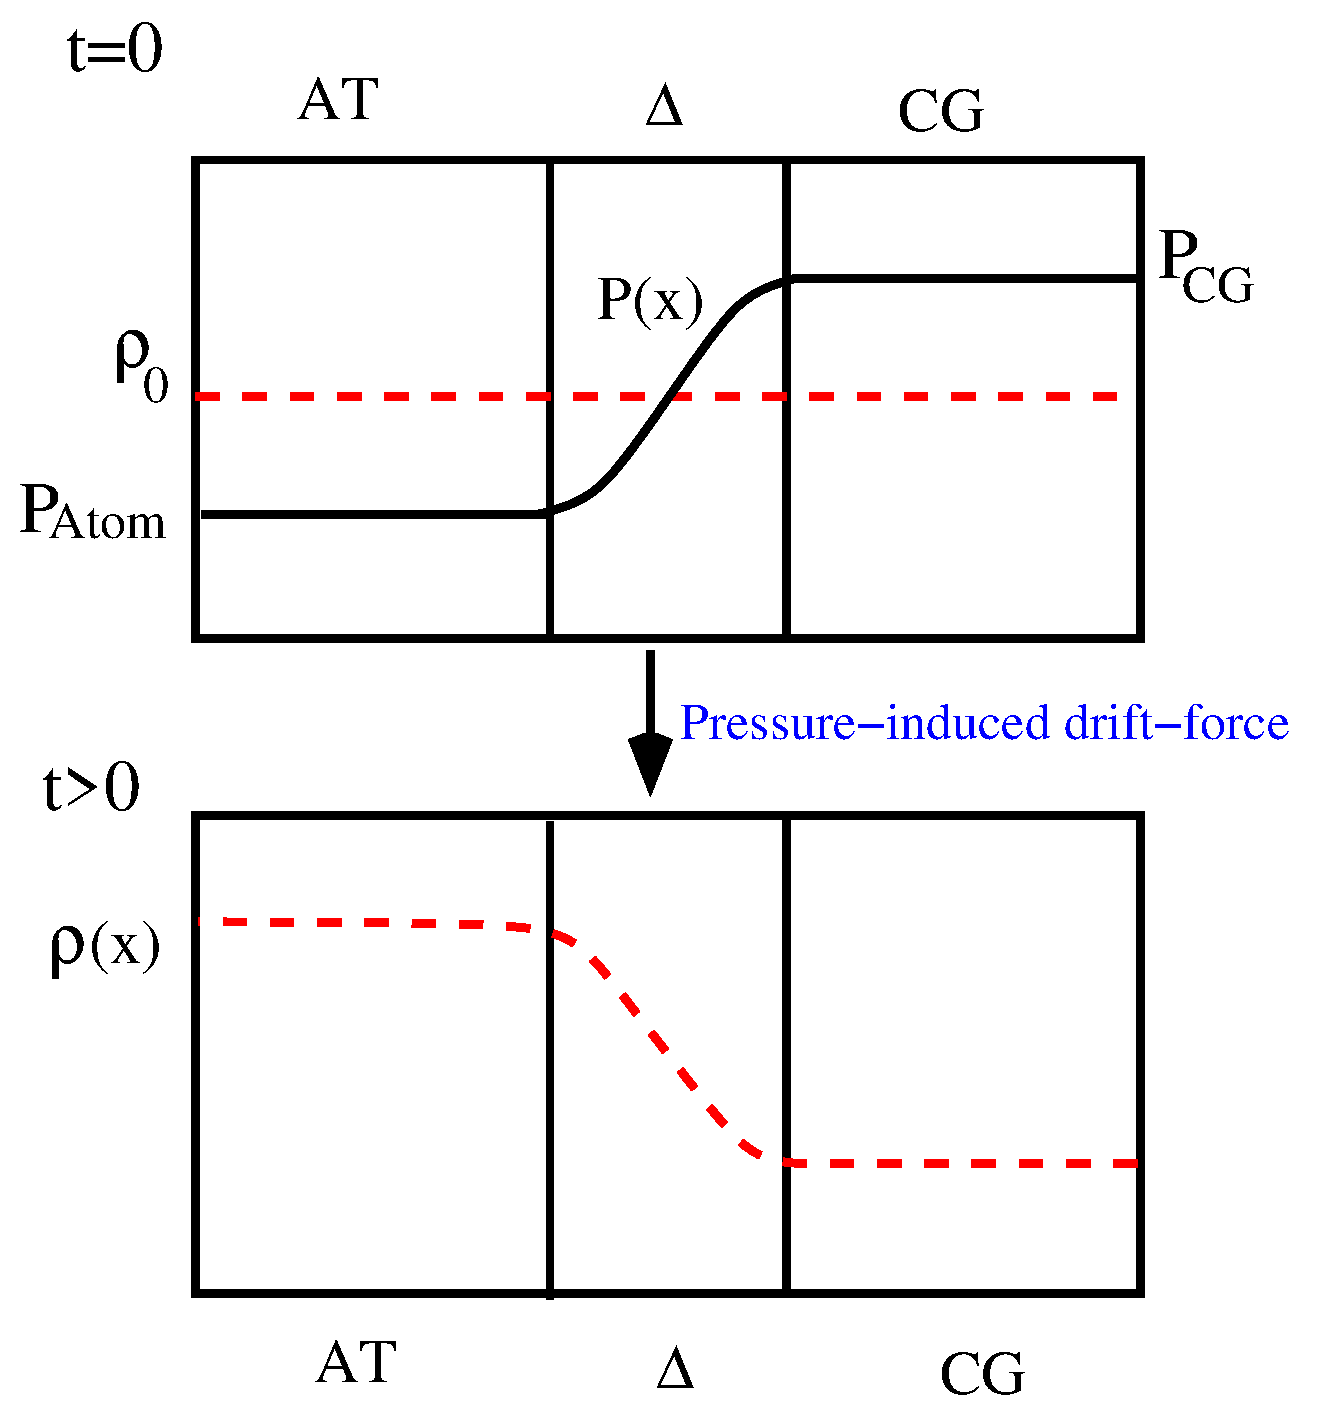
\includegraphics[angle=0,width=8cm]{pressure2.eps}
  \caption{The adaptive resolution initial condition, for AT e CG with different pressure (top). As the simulation proceeds a pressure-induced force produces a drift of particle from the high pressure region to the low pressure region leading to an unphysical density profile}
  \label{figpress}
\end{figure} 


As the simulation proceed ($t>0$) the initial condition of uniform density would not be kept because particles are pushed by the high pressure region to the low pressure region by a pressure-induced drift force. This, as a consequence, leads to a non uniform, unphysical density profile. The solution to this problem is the derivation of a ``thermodynamic force'', that is a force derived on the basis of thermodynamic principles, which compensates the pressure-induced drift force. The thermodynamic principles employed here are the following; interfacing AT and CG models in terms of grand potential means :$P_{AT}V\neq P_{CG}V; \kappa_{AT} =  \kappa_{CG}; \rho\neq \rho_{0}$. The reasons to write the thermodynamic relation in terms of grand potential are: {\bf (I)}  the grand potential is the natural thermodynamic potential when interfacing open systems, that is systems which can exchange particles (the AT and CG are open to each other); {\bf (II)} one can deal directly with the pressure (to which we have direct access) as a natural thermodynamic quantity to correct/adjust in order to obtain equilibrium. In this context the thermodynamic force ${\v F}^{\textrm{th}}(x)$ must be such that: 
\begin{equation}
\left[P_{AT}+ \frac{\rho_{0}}{M_\alpha}\int_{\Delta} {\v F}^\text{th}(x)\,\text{d}x\right] V =P_{CG}V; \quad\kappa_{AT} =  \kappa_{CG}\quad \text{at}\quad\rho=\rho_{0}.
\label{thf}
\end{equation}
The relation above express the situation of a subsystem (e.g.) AT, in equilibrium with a reservoir (e.g.) CG, despite $P_{AT}\neq P_{CG}$ and
(most likely) $\mu_{AT}\neq\mu_{CG}$ (but with no need of specifying either $\mu_{AT}$ or $\mu_{CG}$. In essence, the thermodynamic work generated or adsorbed by ${\v F}^{\textrm{th}}(x)$ removes the differences and assure equilibrium. The explicit expression of ${\v F}^{\textrm{th}}(x)$ is:
\begin{equation}
{\v F}^{\textrm{th}}(x)=\frac{M}{\rho_{0}}\nabla P(x)
\label{explexpr}
\end{equation}
that is at $\rho=\rho_{0}$, Eq.\ref{explexpr} expresses the force on a molecule with mass $M$ balancing the pressure-induced force, $-\nabla P(x)$.
However $P(x)$ is not directly accessible from the simulation and would require a large number of additional runs which would make the procedure computationally not efficient (or as efficient as that of determining $\mu(x))$. For this reason a linear approximation for $P(x)$ is used instead:
\begin{equation}
P(x)\approx P_{AT}+\frac{M_{\alpha}}{\rho_{0}\kappa}[\rho_{0}-\rho(x)]
\label{linearapp}
\end{equation}
where $\rho(x)$ is density generated by the pressure-induced drift-force. Next the thermodynamic force is obtained via an iterative (fastly converging) procedure, as:
\begin{equation}
{\v F}_{k+1}^{\textrm{th}}(x)={\v F}_{k}^{\textrm{th}}(x)-\frac{M_{\alpha}}{[\rho_{0}]^{2}\kappa}\nabla\rho_{k}(x)
\label{iter}
\end{equation}
with $\rho_k(x)$ density profile obtained by the application at the $k$-th iteration of the ${\v F}_k^{\textrm{th}}(x)$.
As a consequence the adaptive coupling, in terms of force acting on the molecule, e.g., $\alpha$ is modified, from ${\v F}_{\alpha}=\sum_{\beta}{\v F}_{\alpha\beta}$ of Eq.\ref{force} to:
\begin{equation}
{\v F}_{\alpha}=\sum_{\beta}{\v F}_{\alpha\beta}+{\v F}^{\textrm{th}}(x_{\alpha}).
\label{mody}
\end{equation}
 It is interesting to note that since $\left({\frac{\partial\mu}{\partial\rho}}\right)_{V,T}=\frac{1}{[\rho]^{2}\kappa}$, we can conclude that this procedure is conceptually equivalent to that labelled (ii) in the previous section, but with the advantage of a much higher computational efficiency.
The approach outlined in this section has been named ``effective Grand Canonical'' because has the characteristic of a standard Grand Canonical system regarding the coupling to a particle reservoir and because the particle number fluctuations in the AT e CG region are preserved. However is an ``effective'' approach because one does not have a direct access to the chemical potential $\mu$ (key quantity for a formal derivation of the partition function in the Grand Canonical ensemble) and because the particle reservoir is finite. The application to liquid water at ambient conditions \cite{prlgc} and to water-methanol mixtures \cite{debash} has proven that the method gives very accurate numerical results if compared with the (by far more expensive) full AT simulations of reference. This means that regarding the computational as well as conceptual robustness of the method the level reached is highly satisfying, however in this work we attempt to define a path to a further systematic improvement, focusing on the reproduction of properties in the transition region $\Delta$.
This is reported in the next section.

\section{Second order correction to the coupling force}
The transition region $\Delta$ has a role of a filter that allows molecules to transit from one region to the other without perturbing the equilibrium of the AT and CG region. While properties in the AT and CG region have a physical meaning, $\Delta$ does not have any physical meaning but represents only a computational convenient tool. In this sense, what is relevant is that quantities  as the $g(r)$, $\kappa$ and the local particle number fluctuations are the same in the AT and CG region (and in turn equal to those of a reference full AT simulation), but it is not necessary that they are same in $\Delta$.
The only significant requirement in $\Delta$ is that the average particle density is the same as in AT and CG region; in fact depletion or increasing of density in $\Delta$ would create artifacts in the AT and CG region. The proper behaviour of the density in $\Delta$ is assured by the application of 
${\v F}^{\textrm{th}}(x)$. However, if there exists a systematic procedure which allows, without massive additional computational costs, also for the $g(r)$, $\kappa$ and the local particle number fluctuations to properly behave in $\Delta$ (that is to be as in the AT and CG region) and assures global thermodynamic equilibrium, then the coupling will be much smoother and would avoid the possibility of any artifacts at the boundaries of the various regions; moreover, by construction, the numerical accuracy should be higher also in the AT and CG region. In the following we show an approach which fulfills the requirements above. To do so, we extend the coupling formula: ${\v F}_{\alpha}=\sum_{\beta}{\v F}_{\alpha\beta}+{\v F}^{\textrm{th}}(x_{\alpha})$, by adding a further force, which assures that the $g(r)$ in $\Delta$ is the same as in the AT and CG region, thus preserves $\kappa$ and the particle number fluctuations without perturbing the thermodynamic equilibrium. We will refer to such an approach as {\it ``second order correction''}; this, because while ${\v F}^{\textrm{th}}(x)$ is based on the correction of the first momentum of the probability distribution of the system in phase space $\rho(x)$, the new additional term is derived as a correction to the second momentum of the distribution, $g(r)$. The technical details of the procedure and the numerical results are shown is the next sections. Finally, we show that the correction to the $g(r)$ represents also a conceptual advancement; in fact it implies that, at least at the level of the COM-COM $g(r)$, the AT region is fully equivalent to a subsystem embedded in a larger full AT bath. That is a natural Grand Canonical ensemble and this it gives more solid formal basis to the approach. 


\section{Determination of the force}
The additional force which should be added up to the thermodynamic force in order to have a $g(r)$ in $\Delta$ as in the AT and CG region must satisfy the following requirements: {\bf (a)} it should act only in $\Delta$; {\bf (b)} it should not perturb the properties of the AT and CG region and the overall equilibrium of the system. In order to fulfil the requirements  above we have developed a scheme whose sequential steps are reported below.\\
{\bf (1)} we proceed to the determination of ${\v F}^{\textrm{th}}(x)$ as reported in the previous section, according to the procedure of Ref.\cite{prlgc}. This will assure us to have the same $g(r)$ in the AT and CG, but not in $\Delta$.\\
{\bf (2)} we correct the interpolation formula on the force by a force correcting the $g(r)$ in $\Delta$:
\begin{align}
  \v F_{\alpha\beta} = w_\alpha w_\beta\v F^{\textrm{AT}}_{\alpha\beta} + [1-w_\alpha w_\beta]\v F^{\textrm{CG}}_{\alpha\beta} + w_\alpha w_\beta (1-w_\alpha w_\beta)\v F_{\alpha\beta}^{\textrm{rdf}}.
\label{grf}
\end{align}
The $g(r)$ correction force $\v F^{\textrm{rdf}}$ is determined by the IBI scheme which in this case is: 
\begin{align}\label{eqn:ibi}
  U^{\textrm{rdf}}_{k+1}(r) = U^{\textrm{rdf}}_k(r) +
  k_B T\ln\bigg[
  \frac{g_k(r)}{g_{\textrm{AT}}(r)}
  \bigg]
\end{align}
where $U^{\textrm{rdf}}(r)$ is the pairwise correction potential
applied to the molecule in $\Delta$. The force is
calculated by
\begin{align}
  \v F^{\textrm{rdf}}_{\alpha\beta} = \v F^{\textrm{rdf}}(\v r_{\alpha\beta})
  = -\nabla_{\v r}\,U(r_{\alpha\beta}).
\end{align}
The $g_{\textrm{AT}}(r)$ is the target AT $g(r)$ that the hybrid
region should reproduce, and $g_k(r)$ is the hybrid radial distribution function of the $k$-th
iteration.  The initial guess of the potential is chosen as the
potential of mean force
\begin{align}\label{eqn:pmf}
  U^{\textrm{rdf}}_0(r) = -k_BT \ln g_{\textrm{AT}}(r).
\end{align} 
The prefactor $ w_\alpha w_\beta (1-w_\alpha w_\beta)$ is chosen such that the force acts only between molecules in $\Delta$. In order to be sure that this is indeed the case we have also slightly modified the switching function $w(x)$ from the expression of Eq.\ref{eqn:old-w} to the following:
\begin{align}\label{eqn:new-w}
  w(x) =
  \left\{
    \begin{array}{lcl}
      1 &\quad& x < d_{\textrm{AT}}\\
      1  && d_{\textrm{AT}} < x < d_{\textrm{AT}} + r_c\\
      \cos^2\big[\frac{\pi}{2(d_{{\Delta}} - r_c)} (x - d_{\textrm{AT}} - r_c)\big] && d_{\textrm{AT}} + r_c < x < d_{\textrm{AT}} + d_{{\Delta}} \\
      0 && d_{\textrm{AT}} + d_{{\Delta}}  < x.
    \end{array}
  \right.
\end{align}
$d_{\textrm{AT}}$, $d_{{\Delta}}$ and $x$ are the same as in Eq.\ref{eqn:old-w}, while $r_c$ is the cut-off
radius; in this work $d_{{\Delta}} \geq 2r_c$.  This definition of $w(x)$, essentially consists in considering an extension of the transition region to part of the AT region (according to the cut off radius $r_c$ (about $0.90\textsf{nm}$); see also Fig.\ref{adapt-wat}). This assures that $\v F^{\textrm{rdf}}(\v r_{\alpha\beta})$ acts only between molecules which are interacting via hybrid resolution.\\
% from the conceptual point of view the new $w(x)$ does not have any further implication.\\
{\bf (3)}  Applying the force obtained by the IBI will correct the $g(r)$ in the hybrid region, however,
the density profile of the system will be disturbed.
To fix this problem, we proceed by performing an additional iteration on the thermodynamic force (TFI) which corrects the density profile,
followed by an IBI step to correct the possible perturbation
of the $g(r)$ due to the the previous iteration of the thermodynamic force.
Therefore, the resulting scheme consists of an iterative
Boltzmann inversion-thermodynamic force iteration correction loop
(IBI-TFI correction loop) to reproduce the correct density
profile and $g(r)$ in $\Delta$ at the same time, (see Algorithm~\ref{algo:1}). 

\algsetup{indent=2em}
\begin{algorithm}
  \caption{IBI-TFI correction loop}
  \label{algo:1}
  \begin{algorithmic}[1]
    \REQUIRE {${\v F}^{\textrm{th}}_{0}$ and $\v F^{\textrm{rdf}}_{0}$}
    \STATE $\v F^{\textrm{th}} \leftarrow \v F^{\textrm{th}}_{0}$, $\v F^{\textrm{rdf}} \leftarrow \v F^{\textrm{rdf}}_{0}$
    \REPEAT
    \STATE $\v F_1^{\textrm{rdf}} \leftarrow \v F^{\textrm{rdf}}$
    \FOR {$k=1$ to $N_{\textrm{IBI}}$}
    \STATE AdResS simulation using ${\v F}^{\textrm{th}}$ and $\v F_k^{\textrm{rdf}}$
    \STATE calculate hybrid RDF $g_k(r)$
    \STATE $U^{\textrm{rdf}}_{k+1}(r) \leftarrow U^{\textrm{rdf}}_k(r) +
    k_B T\ln\big[
    \frac{g_k(r)}{g_{\textrm{AT}}(r)}
    \big]$
    \STATE $\v F_{k+1}^{\textrm{rdf}}(\v r) \leftarrow -\nabla_{\v r}\,U^{\textrm{rdf}}_{k+1}(r)$
    % \STATE update the RDF correction force by \eqref{eqn:ibi}                                                                     
    \ENDFOR
    \STATE $\v F^{\textrm{rdf}} \leftarrow \v F_{N_{\textrm{IBI}}+1}^{\textrm{rdf}}$
    \STATE $\v F_1^{\textrm{th}} \leftarrow {\v F}^{\textrm{th}}$
    \FOR {$k=1$ to $N_{\textrm{TFI}}$}
    \STATE AdResS simulation using $\v F_k^{\textrm{th}}$ and $\v F^{\textrm{rdf}}$
    \STATE calculate density $\rho_k(x)$
    \STATE $\v F_{k+1}^{\textrm{th}}(x) \leftarrow \v F_k^{\textrm{th}}(x)
    - \frac{M}{\rho^2_0\kappa_T}\nabla\rho_k(x)$
    % \STATE update thermodynamic force by \eqref{eqn:tfi}                                                                          
    \ENDFOR
    \STATE ${\v F}^{\textrm{th}} \leftarrow \v F_{N_{\textrm{TFI}}+1}^{\textrm{th}}$
    \UNTIL {both ${\v F}^{\textrm{th}}$ and $\v F^{\textrm{rdf}}$ are converged}\\
    ${\v F}^{\textrm{th}}_0$ is determined following the procedure of Ref.\cite{prlgc}, the initial guess, $\v F^{\textrm{rdf}}_{0}$ is the potential of mean force. The structure of the Algorithm~\ref{algo:1} is rather simple though efficient: 
    in the outermost loop, the IBI and TFI are executed
    consequently, with fixed number of iterations $N_{\textrm{IBI}}$ and $N_{\textrm{TFI}}$,
    respectively. In practice, the TFI converges faster than IBI, so
    $N_{\textrm{TFI}} = 2$ and $N_{\textrm{IBI}} = 50$ provides results with satisfying accuracy.
  \end{algorithmic}
\end{algorithm}
In the next section we will show the application of the method to the case of liquid water at 
ambient condition as in Ref.\cite{prlgc}. We will show that higher accuracy regarding the $g(r)$ and the particle number fluctuation in $\Delta$ 
can be reached and that basic thermodynamic relations (as the Grand Potential) are not perturbed by the additional correction on the forces.

\section{Application to Liquid Water}
Fig.\ref{adapt-wat}, shows the AdResS set up for a system consisting of liquid water at ambient conditions (as in Ref.\cite{prlgc}) to which we have applied the procedure reported in the previous section (technical details of the simulation can be found in the Appendix). Here we show the numerical results for liquid water and prove that our approach represents a successful refinement of the original method of Ref.\cite{prlgc}. 
\begin{figure}
  \centering
  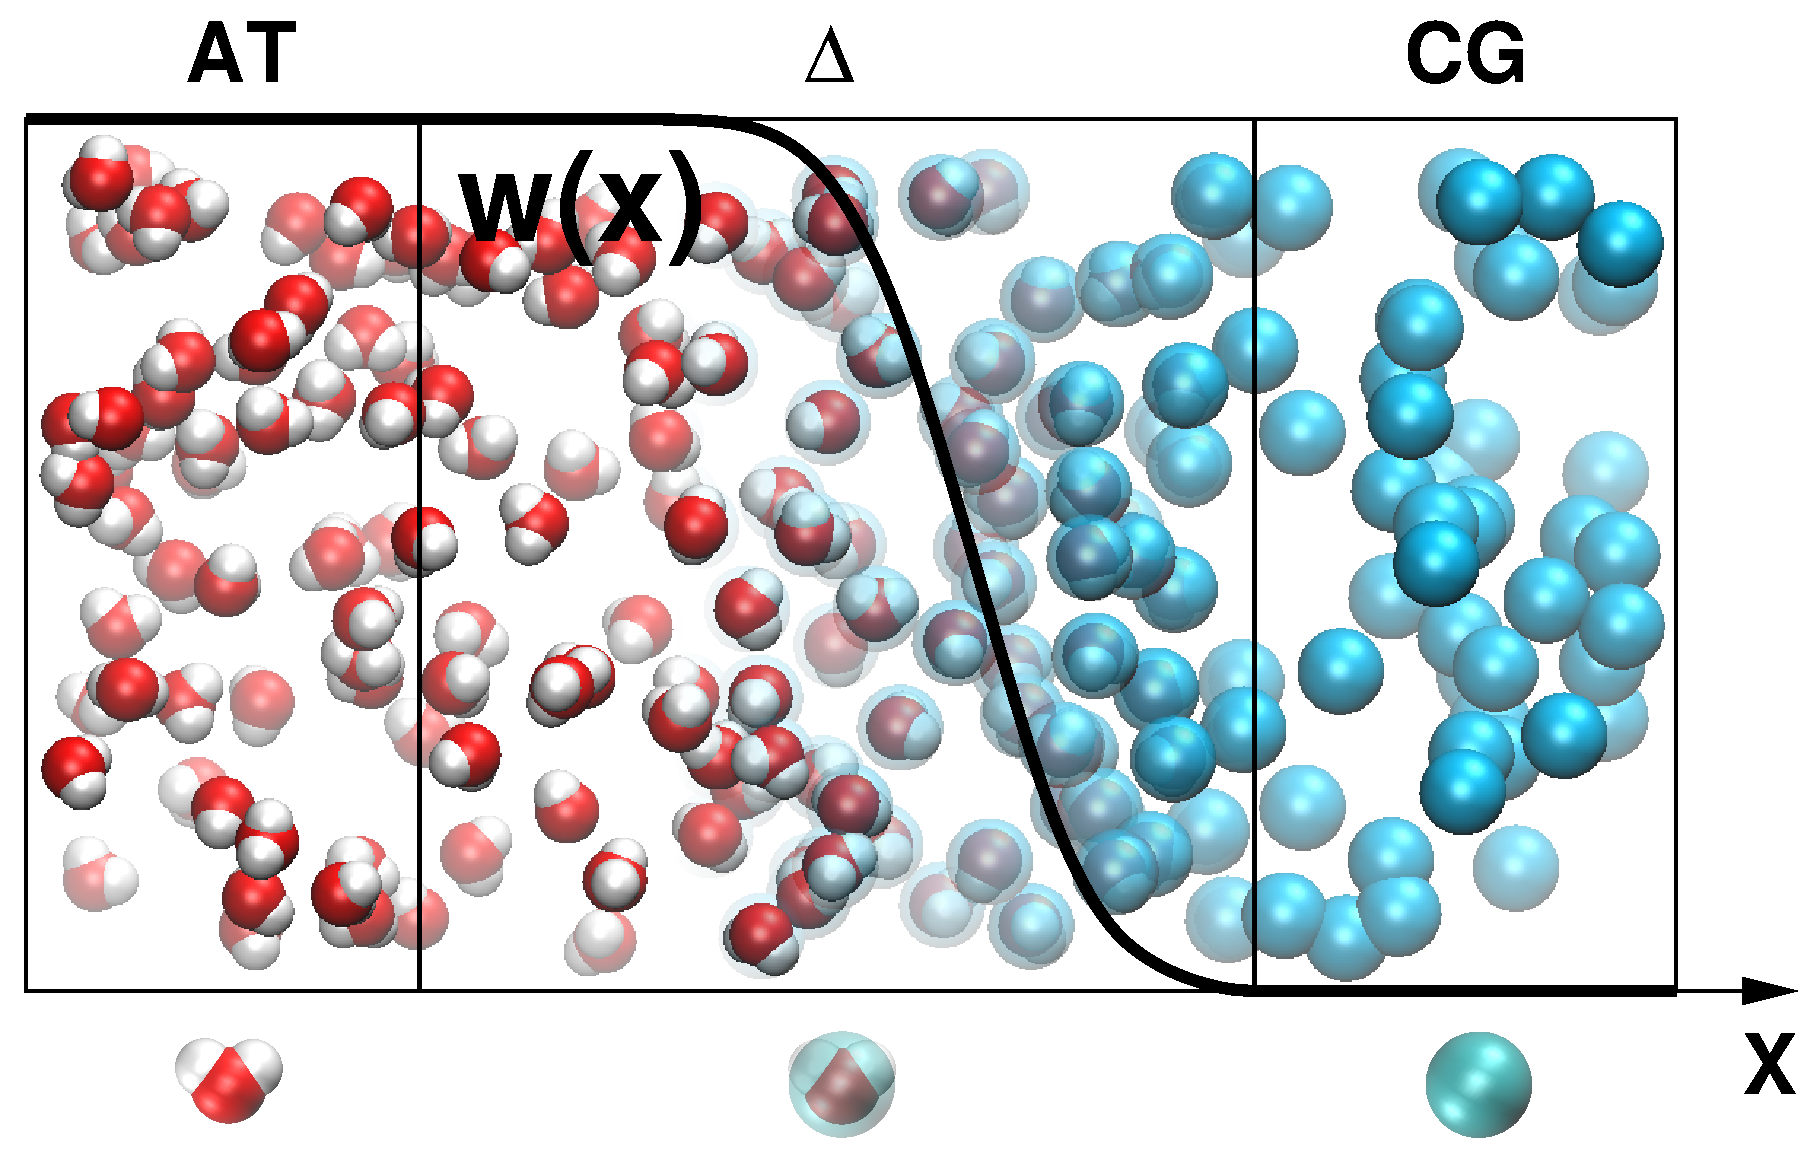
\includegraphics[angle=0,width=10cm]{adapt-wat.eps}
  \caption{Schematic representation of the adaptive simulation box for water where the new proposed $w(x)$ is plotted. Essentially, the $\Delta$ region include a part with full AT resolution. This makes sure that $\v F^{\textrm{rdf}}(\v r_{\alpha\beta})$ acts only between molecules which are interacting via hybrid resolution. The new form of $w(x)$ does not have any further consequence on the system. The $\Delta$ region considered here is, for technical reasons, larger than the AT and CG region; in fact, a $\Delta$ region, larger than the AT and CG region, for the adaptive process is a {\it ``worst case scenario''}. If the approach proposed here, works well with a small AT and CG region (for which a relatively larger $\Delta$ region is a strong perturbation), then it will work well the case where such two regions are much larger than $\Delta$.}
  \label{adapt-wat}
\end{figure}
Fig.\ref{fig:tmp4} shows the $g(r)$ in the $\Delta$ region after the IBI-TFI iteration loop is applied. The agreement with the reference all atom calculation is highly satisfactory. Moreover, the comparison with the results obtained employing the thermodynamic force only (as in Ref.\cite{prlgc}) shows that the additional force, $\v F^{\textrm{rdf}}$, proposed here allows for a sizeable improvement of the structural consistency across the simulation box. The accuracy reached in this case becomes more evident if one considers the $g(r)$ calculated locally in subregions of $\Delta$ across the box; this is shown in Fig.\ref{fig:tmp7}. In the situation where the disagreement on the $g(r)$ in $\Delta$ between the AdResS of Ref.\cite{prlgc} and the reference all atom simulation is larger, that is the central region of $\Delta$ (of about $9.0\, \textsf{nm}$ extension; bottom-left panel in Fig.\ref{fig:tmp7}), the application of the  IBI-TFI correction loop instead significantly improves the situation. 
\begin{figure}
  \centering
  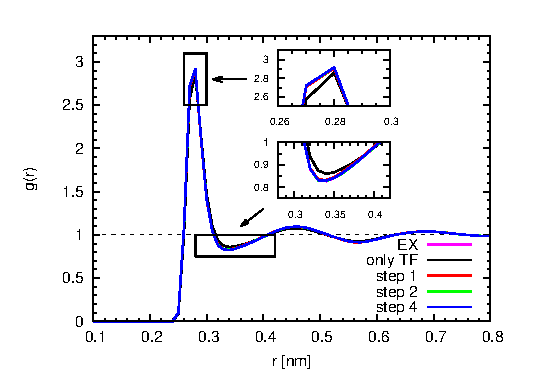
\includegraphics[width=0.69\textwidth]{rdf.eps}
  \caption{The $g(r)$ in $\Delta$ after the IBI-TFI correction loop is applied.  The
    curves obtained after the first, second and the fourth iteration step are represented in red, green and blue solid lines respectively.  The
    curve obtained from the reference explicit all atom calculation (EX) is represented with a solid pink line. However, it must be noted that this latter 
is overlapping with the other lines, and cannot be seen from the
    plot. The curve obtained by applying simply the thermodynamic force correction (only TF),  thus without
    correction on the $g(r)$, is in black. The two insets
    show the details at the
    first peak and the first valley. As it can be seen, after only four iterations $\v F^{\textrm{rdf}}(\v r_{\alpha\beta})$ allows to reproduce, in $\Delta$, with high accuracy the $g(r)$ of the reference full AT calculation.}
  \label{fig:tmp4}
\end{figure} 
\begin{figure}
  \centering
  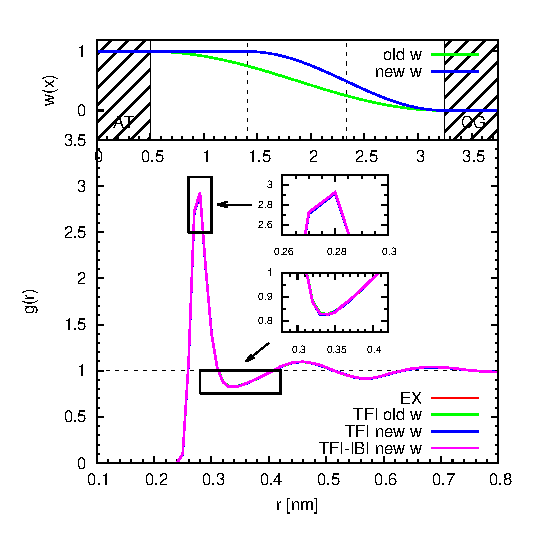
\includegraphics[width=0.49\textwidth]{rdf-ex-cg.eps}
  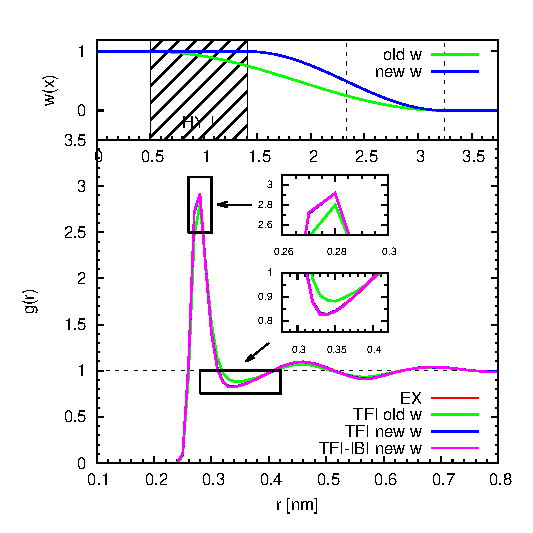
\includegraphics[width=0.49\textwidth]{rdf-425-516.eps}
  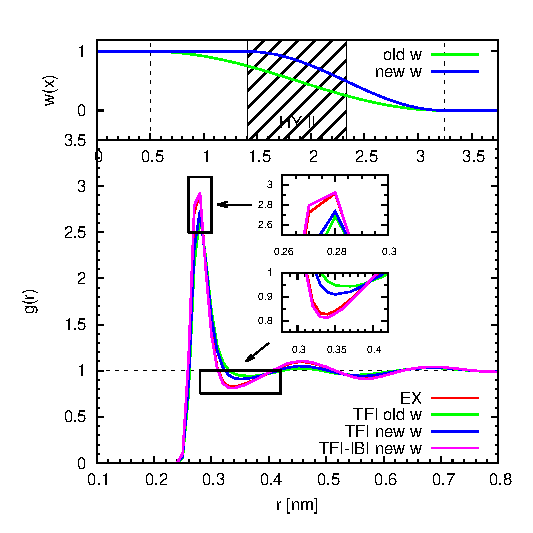
\includegraphics[width=0.49\textwidth]{rdf-516-608.eps}
  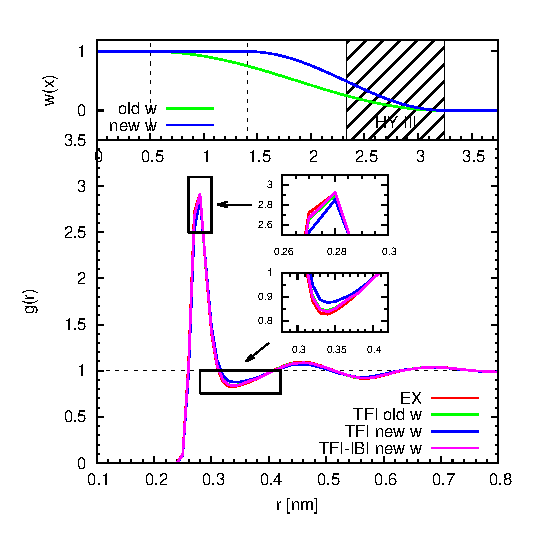
\includegraphics[width=0.49\textwidth]{rdf-608-700.eps}
  \caption{Local $g(r)$'s. The red line is the curve corresponding to the reference explicit (all atom)
    simulation (EX). The curves corresponding to the simulation where only the thermodynamic force is applied, for the case of  
    the old weighting function Eq.\eqref{eqn:old-w} and
    the new weighting function Eq.\eqref{eqn:new-w} are denoted by the
    green and blue line, respectively. The curve obtained by employing the TFI-IBI
    method is represented in pink.
The hybrid region is equally
    divided into three parts: HY I, HY II and HY III, the widths of
    which are roughly equal to the cut-off radius, i.e. 9 \textsf{nm}. 
The top part of each panel shows the region where the $g(r)$ is calculated.
The top-left panel corresponds to the AT and CG case; the top-right to the subregion HY I of $\Delta$, 
closer to the AT region; the bottom-left panel corresponds to the  subregion HY II of $\Delta$, where the level of {\it hybridicity} is the highest, and thus the most delicate case; the bottom-right panel corresponds to the  subregion HY III of $\Delta$, that is closer to the CG region. The insets show the details at the first peak and the first valley.}
  \label{fig:tmp7}
\end{figure}
Next we must show that the IBI-TFI correction loop does not perturb the uniform density profile across the box. Fig.\ref{rho}, shows that at the very first step of the procedure, when $\v F^{\textrm{rdf}}(\v r_{\alpha\beta})$ is applied and ${\v F}^{\textrm{th}}$ is not updated, the density is perturbed. However, despite this initial perturbation, already at the first step of the IBI-TFI iteration loop the density converges towards a uniform profile and that only four steps are required to have a highly satisfied agreement with the results of the explicit all atom reference simulation.
\begin{figure}
  \centering
  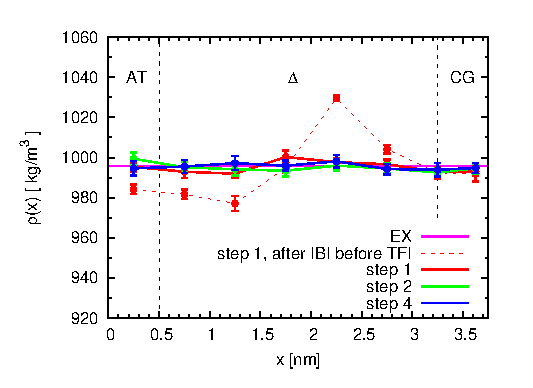
\includegraphics[width=0.59\textwidth]{rho.eps}
  \caption{Particle density across the simulation box. The reference data from the all atom simulation (EX) are reported in pink. The red broken line corresponds to the situation after the correction on the $g(r)$ is applied, but the thermodynamic force is not yet updated. The solid red, green and blue lines represents steps 1, 2 and 4 of the IBI-TFI loop. The agreement with the reference data is highly satisfactory.}
  \label{rho}
\end{figure}
The fast convergence of the iteration loop is also shown in terms of the convergence of the potential correcting the radial distribution function in Fig.\ref{gpot}. More important, the inset shows the convergence of work done by ${\v F}^{\textrm{th}}$: $\int_{\Delta}{\v F}^{\textrm{th}}dx$, as a function of the number of iteration steps. This is an important information because it tells us that the presence in the iterative loop of $\v F^{\textrm{rdf}}(\v r_{\alpha\beta})$ does not perturb the role of the resulting ${\v F}^{\textrm{th}}$ in fulfilling the thermodynamic relation of Eq.\ref{thf} and thus in providing the thermodynamic equilibrium. The difference now, is that also the {\it structural} transition occurs in a much smoother way. A sizeable effect of this smoother transition is shown in Fig.\ref{fluct} where the molecular particle number fluctuation is plotted as a function of the position in $\Delta$.
\begin{figure}
  \centering
  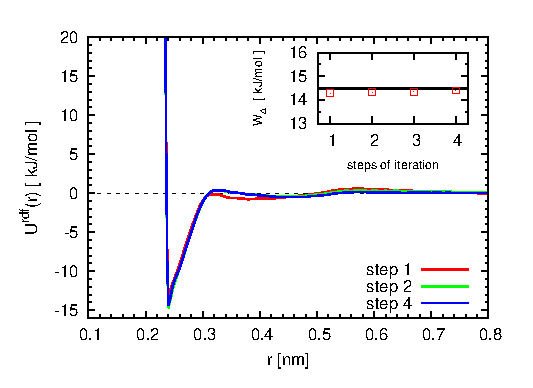
\includegraphics[width=0.59\textwidth]{force-rdf.eps}
  \caption{The plot shows the potential obtained by the IBI iteration to correct the $g(r)$ in $\Delta$; the convergence is shown to be rather fast. The inset shows the convergence towards the target value of the integral $\int_{\Delta}{\v F}^{\textrm{th}}dx$ (i.e. the value obtained without correcting the $g(r)$ in $\Delta$) as a function of the IBI-TFI iteration steps. This is an important results, in fact this quantity represents the work adsorbed or produced in order to have thermodynamic equilibrium in the system; the result shows that the correction force for the $g(r)$ in $\Delta$, does not perturb the overall thermodynamic relation of equilibrium.}
  \label{gpot}
\end{figure}
While the results of the original method of Ref.\cite{prlgc} show an evident deviation from the results of the reference all atom simulation, for the case where the TFI-IBI loop is applied there is a satisfactory agreement and basically the two curves overlap within the error bar. This assures that particle number fluctuations are the same as in the AT and CG region and that no artifact due to wrong fluctuation properties can propagate into the AT and CG region.
\begin{figure}
  \centering
  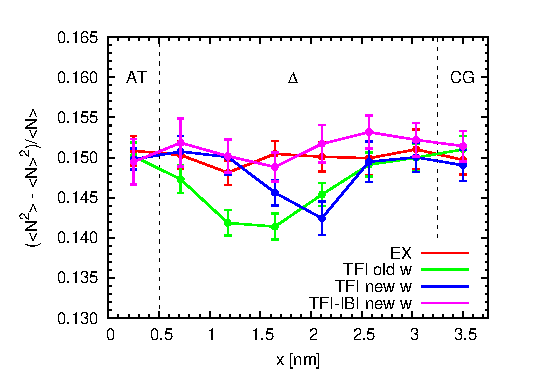
\includegraphics[width=0.59\textwidth]{count.eps}
  \caption{Particle number fluctuation in $\Delta$. The reference data from a full atomistic simulation are reported in red (EX). The green line represents results obtained with the original formulation, blue with the new $w(x)$ but without the application of the TFI-IBI loop, pink the results of the new method.}
  \label{fluct}
\end{figure}


\section{Theoretical Considerations}
Let us consider the dynamics of a system that is subject to the Langevin equation (the thermostat usually employed in the AdResS simulations):
\begin{align}
  \d d\v r_i &= \v v_i\d dt\\
  m_i\d d\v v_i &= [-m_i\xi_i\v v_i + \v F_i]\,\d dt + \sqrt{2\sigma_i}\,\d d\v W_t
\end{align}
where $\d d\v W_t$ is the standard Wiener process.  If the system has a
potential, namely $\v F_i = -\nabla_{\v r_i}U$, then it can be proved that the
Langevin dynamics generates the canonical ensemble:
\begin{align}
  p(\v r_1, \cdots, \v r_N, \v v_1, \cdots, \v v_N)
  \propto \exp\big[
  -\beta \mathcal H(\v r_1, \cdots, \v r_N, \v v_1, \cdots, \v v_N)
  \big]
  % \bigg[
  % \sum_i^N\frac12 m_i\v v_i^2 + U(\v r_1, \cdots, \v r_N)
  % \bigg]
\end{align}
where $\mathcal H$ is the Hamiltonian of the system:
\begin{align}
  \mathcal H(\v r_1, \cdots, \v r_N, \v v_1, \cdots, \v v_N)
  =
  \sum_{i=1}^N\frac12 m_i\v v_i^2 + U(\v r_1, \cdots, \v r_N)  
\end{align}
Let us first consider the case where we have $N_1$
molecules in the atomistic region, $N_2 - N_1$ molecules in the hybrid
region.  Without loss of generality, we assume molecules $1, \cdots,
N_1$ are in the atomistic region, molecules $N_1 + 1, \cdots, N_2$ are
in the hybrid region and $N_2+1, \cdots, N$ are in the coarse-grained
region. The pair $\{\v r_i, \v v_i\}$ of the atomistic representation
denotes the center-of-mass (COM) position and velocity of the $i$-th
molecule. For convenience, we only consider the COM coordinates of the
AT molecule, all the arguments employed here
can be easily extended to treat each atom the the molecule.
We hereby consider the AT region as a subsystem of the whole
system, which is composed by the AT, $\Delta$ and CG
regions. We must always take in mind that our reference system is the full AT case.
Thus the properties of the AT subsystem in AdResS must be the same of the equivalent subsystem in a full AT case.
 If we (hypothetically) fix the coordinates of the molecules in $\Delta$ , according to the definition of $w(x)$ in Eq.\ref{eqn:new-w}, the Hamiltonian in the AT region can be written as
\begin{align}
  \mathcal H^{\textrm{AT}}(\v x_1; \v x_2) =
  \sum_{j=1}^{N_1}\frac12 m_i\v v_i^2 + 
  \sum_{i,j=1}^{N_1}\frac12 U^{\textrm{AT}}(\v r_i - \v r_j) + 
  \sum_{i=1}^{N_1}\sum_{j=N_1+1}^{N_2} U^{\textrm{AT}}(\v r_i - \v r_j) 
\end{align}
We denote the phase space variables: $\v x_1 = (\v r_1, \cdots, \v
r_{N_1}, \v v_1, \cdots, \v v_{N_1})$,  $\v x_2 = (\v r_{N_1+1},
\cdots, \v r_{N_2}, \v v_{N_1+1}, \cdots, \v v_{N_2})$ and
$\v x_3 = (\v r_{N_2+1},
\cdots, \v r_{N_3}, \v v_{N_2+1}, \cdots, \v v_{N_3})$. $\v x_{3}$ denotes the coordinates and velocities of the COM of the molecules in the CG region and for the moment do not enter in our derivation.
Here we can consider $\v x_1$ to be the variable and $\v x_2$ a certain (fixed) external molecular environment. 
According to the Langevin dynamics, we have the conditional probability distribution:
\begin{align}
  p (\v x_1 \vert \v x_2)  \propto
  e^{-\beta \mathcal H^{\textrm{AT}}(\v x_1; \v x_2)}
\end{align}
Accordingly, the phase space distribution of the AT region writes:
\begin{align}
  p(\v x_1) = \int p(\v x_1\vert\v x_2)\cdot p (\v x_2) \,\d d\v x_2
\end{align}
If the distribution $p(\v x_2)$ is equivalent to that of the corresponding region in a full AT reference system, then one can consider the AT region in AdresS to be the equivalent of a subsystem embedded  a very large AT
system.
The crucial question is if $p(\v x_2)$ is equivalent to that of a full AT system. 
Most likely this is not the case, at least for the interpolation scheme plus the thermodynamic force. In fact if one consider $p(\v x_2)$ expanded in terms of its momenta, by performing simulations using the coupling scheme of Eq.\ref{mody}, the first order of $p(\v x_2)$ is correct (i.e. the particle density) but already at the second order, that is the COM-COM radial distribution function, the hybrid region deviates from the other two regions. However, as we have shown in the previous sections, one can add a further corrective force in the hybrid region
and obtain a radial distribution function as that of the AT and CG region. This would mean that the idea of the AT region as a subsystem of a very large AT system, is correct up to the second order in terms of distribution. This we have shown is more than sufficient for numerical accuracy. Moreover, to define a subsystem in a large full AT simulation is formally equivalent to (naturally) define a Grand Canonical set up and thus justifies, in good approximation, our view of the AT region in AdResS as an effective Grand Canonical ensemble.  

\section{Conclusions}
We have proposed an extension of the effective Grand Canonical formulation of the adaptive resolution method. In the adaptive approach, it is important that structural properties and basic thermodynamic quantities in the AT and CG region are the same as in the reference full AT simulation, while the transition region $\Delta$ has no physical meaning and represents only a computational tool to favorite the change of resolution keeping the overall equilibrium of the system. In the original formulation of the effective Grand Canonical AdResS, only the particle density in $\Delta$ is assured to be the same as in the AT and CG region. This requirement is crucial since depletion or excess of particles in $\Delta$ implies a higher/lower density in the AT and CG region and thus a situation different from the reference full AT system.  However if one constructs a systematic procedure which preserves the thermodynamic equilibrium (as in the current formulation) but goes beyond the requirement of density in $\Delta$ and assures that further structural (radial distribution function) as well as thermodynamic properties (isothermal compressibility and the related particle number fluctuations) are reproduced in this region, then the transition from AT to coarse-grained resolution (and vice versa) would be even smoother and avoid any possible artifact at the border of the AT and CG region. In this work we have proposed such a procedure. It is based on a loop consisting of correcting the $g(r)$ in $\Delta$ and refine the thermodynamic force for the overall thermodynamic equilibrium. Though computationally more demanding than the original formulation (due to this additional loop), it shows that the smoothness of the transition from one resolution to the other can be systematically improved. While for adaptive resolution simulations of liquid water the accuracy of the original formulation is already highly satisfactory, there may exist systems where the importance of the particle number fluctuations in $\Delta$ can play a central role for a smooth transition. This is the case of larger molecules or polymers \cite{jstatphyskurt} and certainly for the quantum/path integral version of the adaptive method \cite{adolfo1,adolfo2,raffaello}, since this latter is based on the ring-polymer representation of atoms and molecules. Moreover we have given theoretical arguments that show how the agreement on the $g(r)$ in $\Delta$ justifies, up to the second order, the view of the AT system in AdResS as an equivalent subsystem in a large full AT system and thus gives more solid arguments to the interpretation of the AT region as an effective Grand Canonical ensemble. 

\section{Acknowledgment}
We thank Sebastian Fritsch for the help in guiding us in the use of the AdResS code at the initial stage of the project.\\ 
This work was partially supported by the Deutsche Forschungsgemeinschaft (DFG) with the Heisenberg grant provided to L.D.S (grant code DE 1140/5-1) and by......provided to H.W and C.S.

\section{Appendix}
The testing system contained 3456 SPC/E \cite{berendsen1987missing}
water molecules in a $7.50\textsf{nm}\times 3.72\textsf{nm}\times
3.72\textsf{nm}$ periodic box. The system was divided along the $x$ direction
into one atomistic region of width $1.00\textsf{nm}$ and one
coarse-grained region of width $1.00\textsf{nm}$ connected by two
hybrid region of width $2.75\textsf{nm}$. The simulation was made at
room temperature of $300\textsf{K}$. The time step was $\Delta t =
0.002\textsf{ps}$. The cut-off radius $r_{c}$ used for all interactions was
$0.90\textsf{nm}$. The electrostatic interaction method used for the
atomistic region was the reaction field method. All simulations were
performed by MD simulation software Gromacs \cite{gromacs}
and VOTCA \cite{ruehle2009versatile}.




\bibliography{ref}{}
\bibliographystyle{unsrt}

\end{document}
